\chapter{Introduction}
\label{cha:introduction}
\epigraph{
  \hypersetup{linkcolor=bgwhite}
  This thesis will explore the possibility of creating an anomaly detection for
  non-linear time series. In its broadest sense this means finding unusual,
  unexpected, or new patterns in a given dataset. In this introductory chapter,
  the motivation for searching for anomalous behaviour is described alongside
  the requirements for a general anomaly detection algorithm. Because many
  physical systems that are of interest for an outlier detection are non-linear
  and possibly even show \emph{chaotic} behaviour, a brief definition of
  chaotic time series is given, followed by three concrete exemplary datasets.\\
  The problem of detecting anomalies has been
  studied in many fields, which has lead to a great number of different
  approaches to the problem, some of which will be summarized in
  Chapter~\ref{cha:anomaly_detection};  Chapter~\ref{cha:neural_networks}
  introduces Neural Networks and their potential for predicting arbitrary time
  series, their implementation is described in Chapter~\ref{cha:implementation}
  and finally Chapter~\ref{cha:results} presents the so-called \emph{echo
  state network} applied to the three datasets that were introduced earlier.
  \hypersetup{linkcolor=linkblue}
}


\section{Motivation}
\label{sec:motivation}

The identification of unusual or aberrational behaviour is treated in many
other scientific fields:  The purpose of magnetic resonance imaging (MRI) is to
find tissues that are not expected to be found at a certain location in the
body, indicating a tumor. Biology studies genetic anomalies, \emph{mutations},
that can cause either illness or an increased chance of survival of an
individual.  Engineers monitor their equipment to detect early warning signs
before a machine breaks.  Banks try to identify fraudulent transactions based
on peculiarities in credit card data.  Anomalies in weather data can give early
hints on upcoming droughts, storms or other weather phenomena.  DNA sequence
mutations, engine monitoring, fraud detection, and weather data are examples of
sequential datasets that can be regarded as time series.  Detecting outliers in
time series can help prevent undesired behaviour or develop an early warning
systems.  With the growing amount of data that is being produced in many
different fields it becomes infeasible to manually analyze the given datasets.
It is therefore highly desirable to create an anomaly detection that is as
general as possible with regard to the data it can successfully process.\\

A field which could benefit immensely from an automated anomaly detection is
ocean modelling.  Large scale, high resolution simulations that cover the whole
Earth with more than 30 different variables such as temperature, velocity, and
density easily take up tens of gigabytes for a single time step. The vast
majority of the simulated ocean, much like the real ocean, is almost completely
unexplored.  Potentially unknown physical behaviour that could be hidden in
these datasets could be found by an automated outlier search. An example of
such an anomaly is the state changing ocean current called \emph{Kuroshio} on
the coast of Japan.  In irregular periods of several years it changes from an
elongated to a contracted state. This phenomenon has just recently come to the
attention of the scientific community and its origin is subject of vivid
debate. A detection of similar anomalies would be a very interesting finding in
itself, but it could also contribute to a deeper understanding of the Kuroshio
anomaly and the ocean circulation as a whole.

A large part of the anomaly detection model consists of a Neural Network. They
have been successfully applied to a very large number of different problems,
but have not yet found their way into the standard analysis tools of climate
scientists. With this thesis we hope show what could be achieved with an AI
driven approach to climate research.



\section{Defining Normality}%
\label{sec:defining_what_is_normal}

This thesis aims for the creation of an automatic detection algorithm that can
analyze large spatio-temporal datasets. We assume no prior knowledge about the
physics that produces the data, so there is no knowledge about the kind of
anomaly that we are looking for.  This requires to define what is
{\em normal}, so that everything that looks significantly different than this
norm can be treated as anomalous.  In time series this norm can be defined by
trying to predict the future evolution based on a previously observed history.
This means that we want to create a model that consumes an input sequence
$\mathbf{u}$ and returns a prediction sequence $\mathbf{y}$ (formal description
in Sec.~\ref{sub:prediction}):
\begin{equation}
  \mathbf{y} = F(\mathbf{u})
\end{equation}
The acquired prediction can subsequently be compared with the true values that
the sequence takes on for the predicted interval.  As soon as a reasonably good
prediction is made, the actual detection of an anomaly becomes quite simple.
Based on the degree of the deviation of prediction and truth, an \emph{normality
score} (Sec.~\ref{sub:anomaly_score}) can be calculated to define how large the
deviation must be in order to count as an anomaly.


\section{Applications}%
\label{sec:applications}

The generality of the algorithm is showcased with three exemplary datasets.
Each of the datasets will be described in more detail in the sections
\ref{sec:mackey_glass_system}-\ref{sec:kuroshio} of this chapter, but in short
they can be summarized as follows.

The first test-problem is a scalar chaotic system governed by the Mackey-Glass
equation. Scalar systems will further be referred to as zero-dimensional (0D).
%
Next, the algorithm is applied to a real-world example: climate records that
were obtained from Greenland ice-cores and include well known anomalies that
are called Dansgaard-Oeschger (DO) events.  The time series consists of two
markers that are fed to the detection algorithm, which is slightly increasing
the complexity of the task. The DO dataset can be regarded as a very small
one-dimensional (1D) system, as the input is a vector with two components.
%
Finally, the performance of the algorithm on a 2D system is analyzed. It
consists of a sequence of simulated sea surface height (SSH) images of the
previously mentioned Kuroshio region next to Japan. A successful anomaly
detection on this dataset would equate to an automated novelty detection in a
vast amount of climate data.



\section{Outline}%
\label{sec:outline}

The second chapter gives a brief introduction to what anomalies are, describes
some frequently used detection techniques, and defines the goal of the
predictive anomaly detection that will be used.  In the third chapter, whose
subject is Neural Networks, the theoretical background that is needed to
implement an automated time series prediction is laid out. It includes an
introduction to feedforward and recurrent networks before describing a new
machine learning concept called \emph{reservoir computing} (RC). The RC
approach, in comparison to traditional ML, is less computationally expensive
and was shown to be capable of forecasting chaotic systems surprisingly well in
a paper by [\cite{jaeger2004}] and for the first time for high dimensional
datasets by [\cite{pathak2018model}]. The implementation of the algorithm is
sketched in chapter~\ref{cha:implementation} and the results are presented in
chapter~\ref{cha:results}.


\newpage
\section{Chaotic Time Series}%
\label{sec:chaotic_time_series}

Time series are characterized by a chronological sequence of events.  In this
thesis only discrete time series, where each data point is associated with a
timestamp, are treated.  The basic components of a \emph{linear} time series are
level, trend, seasonal, and random effects. \emph{Level} is simply the current
value of the series, the \emph{trend} describes the increase and decrease from
one step to another. The \emph{seasonal} component refers to recurring patterns
that can be explained by some kind of seasonal influence like the tides.
\emph{Random} effects describe the statistical fluctuations of the series.
This is a typical linear treatment of the problem of analysing sequences.  The
complex problem is broken down into parts which can be solved individually and
finally linearly recombined.  For {\em non-linear} systems this cannot be done
so easily.  Various physical systems exhibit this non-linear behaviour which
can, under certain conditions, lead to \emph{chaotic} time series.
\begin{quote}{S. H. Strogatz}
  \emph{Chaos is aperiodic long-term behaviour in a deterministic system that
  exhibits sensitive dependence on initial conditions.}
\end{quote}
By aperiodic we mean behaviour that cannot be explained by strictly periodic
effects. There are no random inputs needed for this aperiodicity to occur,
which is suggested by the deterministic nature of the system. Its capricious
behaviour arises from the non-linearity.  The sensitivity to initial conditions
is the most commonly noted feature of chaotic systems.  It means that two
points $x(t)$ and $x(t)+\delta(t)$ that start out infinitesimally close to each
other will quickly diverge and evolve in completely different ways.  Their
separation may initially grow exponentially fast
\begin{equation}
  ||\delta(t)|| \sim ||\delta_0|| e^{\lambda t}.
\end{equation}

In this case the number $\lambda$ is called Lyapunov exponent. In systems where
$\lambda > 0$, one finds chaotic behaviour and the larger $\lambda$ grows the
more sensitive is the system to initial perturbations. The Lyapunov exponent
for the famous Lorenz attractor~[\cite{lorenz1963deterministic}] can be
computationally found to be $\lambda \approx 0.9$.  Chaotic systems are not the
same as \emph{unstable} systems, which also exhibit this sensitivity to initial
conditions. Unstable systems however, diverge towards infinity, while in
chaotic systems $\delta(t)$ is bounded by the radius of the \emph{attractor}.
A formal definition of attractors is out of the scope of this work, but the
interested reader may be referred to the book \emph{Non-linear Dynamics and
Chaos} by [\cite{strogatz}].


\newpage
\section{Mackey-Glass System}%
\label{sec:mackey_glass_system}

The Mackey-Glass (MG) system is a simple \emph{delay} differential equation,
that exhibits chaotic behaviour under certain conditions. It is studied
extensively in non-linear dynamics and serves as a benchmark for chaotic
prediction algorithms. It is defined by

\begin{equation}
  \label{eq:mackey_glass}
  \frac{\partial x}{\partial t} = \beta \frac{x_\tau}{1+x_\tau^n} - \gamma x,
  % discrete:
  %x(n+1) = x(n) + \delta (\frac{0.2x(n+\tau/\delta)}{(1+x(n-\tau/\delta)^{10}} - 0.1x(n))
\end{equation}

where $\beta$ and $\gamma$ are constants and $x_\tau$ denotes the value
$x(t-\tau)$, representing the delay.
\begin{figure}
  \centering
  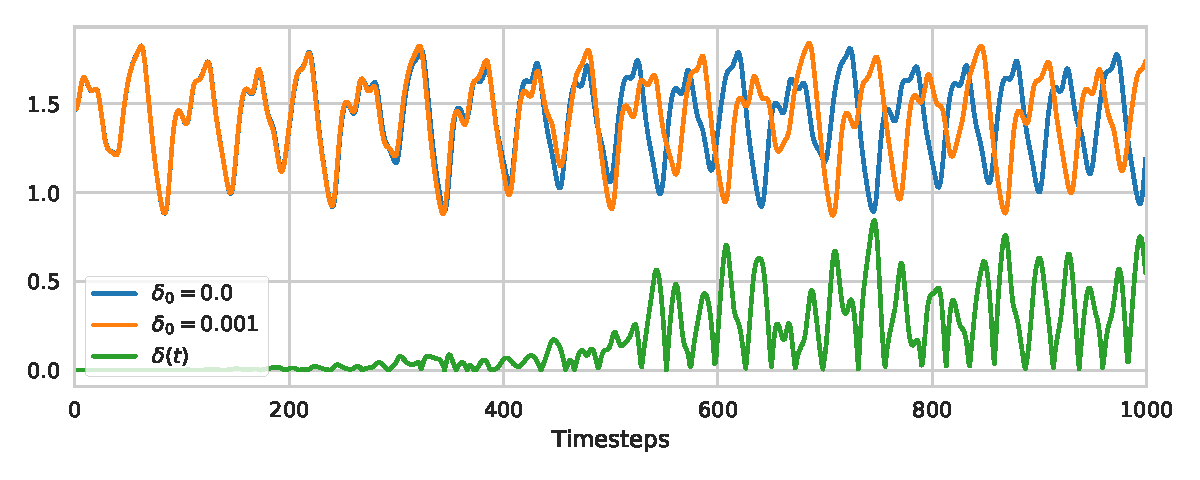
\includegraphics[width=\linewidth]{mackey_glass.pdf}
  \caption{Mackey-Glass time series created from Eq.~\ref{eq:mackey_glass}.  It
    nicely shows the aperiodic behaviour of chaotic time series, which makes it
    difficult to predict the next cycle. The two different evolutions are caused by
    a separation of $\delta_0 = 0.001$. There are no anomalies in the
    sequence. They will be introduced in Sec.~\ref{sec:res_mackey_glass_system}
    by slightly varying $\gamma$ over time.}
  \label{fig:mackey_glass}
\end{figure}
Two sequences that are created by solving Eq.~\ref{eq:mackey_glass} with the
values $\beta = 0.1$, $\gamma=0.2$ and a delay of $\tau=17$ are shown in
Fig.~\ref{fig:mackey_glass}. To solve the MG system initial values of the
length of the delay $\tau$ need to be specified. The two different evolutions
in the plot are created by slightly perturbing the initial values by
$\delta_0$. Additionally the plot shows how the separation $\delta(t)$ of the
two runs evolves. As expected, the peaks of the separation look very much like
an exponential for some time.
The local lyapunov exponent (LLE, [\cite{eckhardt1993}]) of the Mackey-Glass
system was calculated to LLE $\approx 0.01$ by [\cite{sprott}].



\newpage
\section{Dansgaard-Oeschger Events}%
\label{sec:dansgaard_oeschger_events}

During the last glacial period the North Atlantic region was subject to a
number of large climatic fluctuations known as Dansgaard-Oeschger (DO) events.
They describe abrupt increases in surface temperature of up to 15$^\circ$C over
a few decades, followed by a gradual cooling. Automatically detecting DO events
in time series that are obtained from Greenland ice-cores could serve as an
interesting benchmark for this anomaly detection method. Additionally the
dataset serves as a first step towards higher dimensional time series.

The INTIMATE project (INTegrating Ice-core, MArine, and TErrestrial records)
has recently managed to extract records of the DO events from Greenland
ice-cores that were drilled down to depths of about 3000m and contain climatic
information of the past 100 000 years.  Two different markers that clearly show
DO events are considered here: the so-called $\delta^{18}$O value is directly
linked to past temperatures, while the Ca$^{2+}$ concentration measures dust
content, which can be connected to atmospheric conditions such as the
atmosphere's circulation pattern.

The $\delta^{18}$O value measures the ratio of the lighter oxygen isotope
$^{16}$O and the heavier $^{18}$O in precipitation water [\cite{rasmussen2014}].
Higher temperatures aid the evaporation of water that contains the heavier
oxygen isotope, which means that roughly, one per mill change in $\delta^{18}$O
corresponds to a temperature difference of 1.5-4$^\circ$C.  With Greenland
ice-cores it is possible to resolve annual temperature oscillations as far back
in time as 8000 years. The sequence that is considered here contains annual
means because we are not interested in seasonal changes.

The concentration of Ca$^{2+}$ is essentially a measure of the dust content of
the ice. More dust indicates stronger winds that carried it to Greenland. By
measuring other isotopes it is even possible to determine where the dust comes
from, which gives hints on the atmospheric circulation patterns at the time,
but these isotopes are not considered here.  Fig.~\ref{fig:doevents} shows how
well the Ca$^{2+}$ and $\delta^{18}$O values coincide. Not that the time axis
shows age, so the time moves forward from right to left. The DO events are
indicated by the grey shaded regions.

\begin{figure}
  \centering
  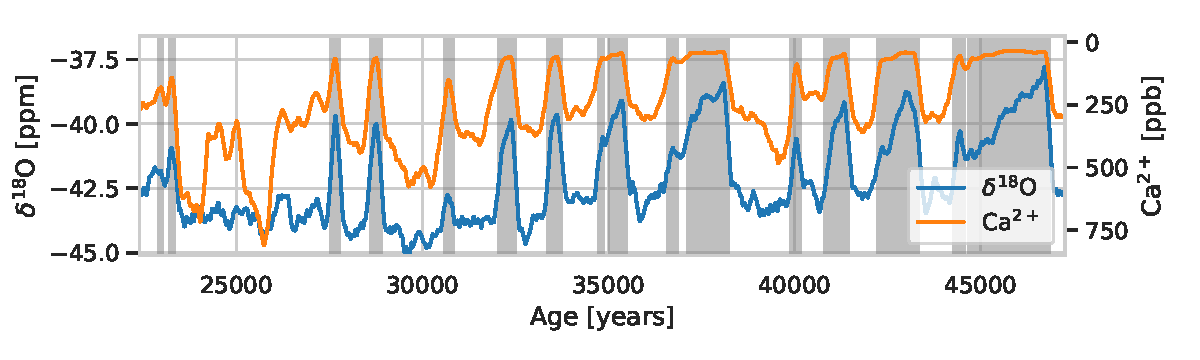
\includegraphics[width=\linewidth]{doevents.pdf}
  \caption{A sample of the $\delta^{18}$O (related to temperature) and
  Ca$^{2+}$ (dust content) sequences.  Dansgaard-Oeschger are marked by the
  grey shaded regions.}
  \label{fig:doevents}
\end{figure}



\newpage
\section{Kuroshio}%
\label{sec:kuroshio}

The Kuroshio [\textsc{japanese: black tide}] is one of the strongest ocean
boundary currents in the world and is the result of the western intensification
[\cite{pedlosky2013ocean}] of the ocean circulation in the North Pacific. The
3-day mean of simulated sea surface height (SSH) data
(Fig.~\ref{fig:kuroshio_snapshot}) shows the Kuroshio and its extension that
reaches into the North Pacific basin. It carries with it large amounts of
energy, nutrients and biological organisms, which have a large impact on the
local and global climate. To make itself even more relevant, the Kuroshio
exhibits a interesting and not yet understood phenomenon. In front of the coast
of Japan it oscillates between two distinct states
(Fig.~\ref{fig:kuroshio_elon_contr}): an elongated (right) and a contracted
state (left).  The transition between the two states typically takes one to two
years and occurs, as it seems, randomly every few years.  In 2017 it
transitioned to its elongated state for the first time in over a decade, as
reported by a Japanese newspaper [\cite{mainichi}]. To the interested reader it
also describes its impact on the local fishing industry as well as on tide
levels and the weather.

\begin{figure}
  \centering
  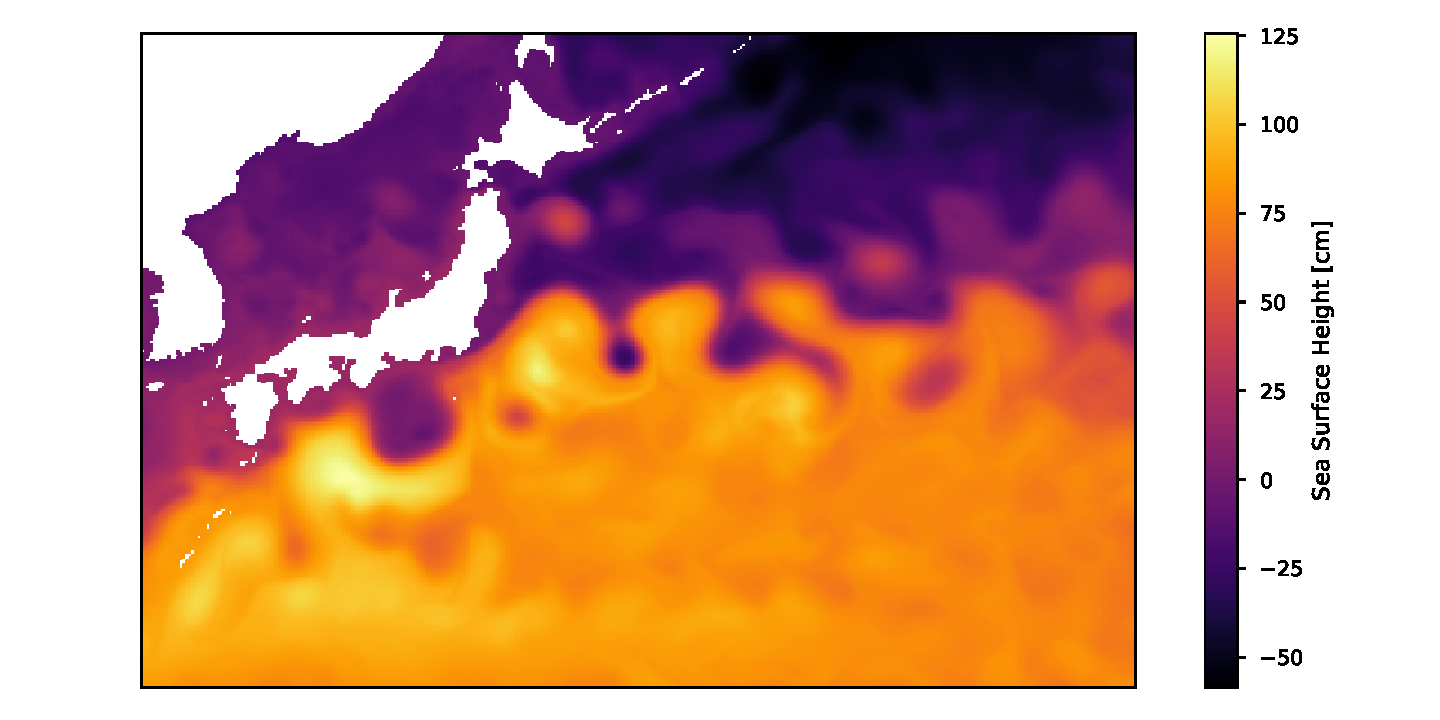
\includegraphics[width=1.05\linewidth]{kuroshio_snapshot.pdf}
  \caption{3-day mean of simulated sea surface height data. The Kuroshio is
  visible at the sharp transition between blue and yellow color. It flows along
  the coast of Japan before turning into the North Pacific basin. The figure is
  created by a 440x290 pixel window of the global simulation domain that is
  3600x2400 pixels large.}
  \label{fig:kuroshio_snapshot}
\end{figure}

The simulations that created the pictures were carried out by \emph{Team Ocean}
at the University of Copenhagen. The \emph{Community Earth System Model} (CESM)
was used to simulate the global domain with a horizontal resolution of
0.1$^\circ$ and 62 depth layers. It writes out 3-day means for all variables,
but in this work only the SSH fields are considered, which results in
images of a total size of 3600 x 2400 pixels. A more detailed
description of the experimental setup can be found in [\cite{poulsen2018}].  As
indicated by Fig.~\ref{fig:kuroshio_elon_contr}, the Kuroshio anomaly was
reproduced in the CESM simulations. The two plots of the elongated and the
contracted state were produced by averaging 200 3-day mean snapshots of the
simulation at different time periods. Taking the difference of them should give
us an intuition for how a successful anomaly detection should look like.\\
\begin{figure}
  \centering
  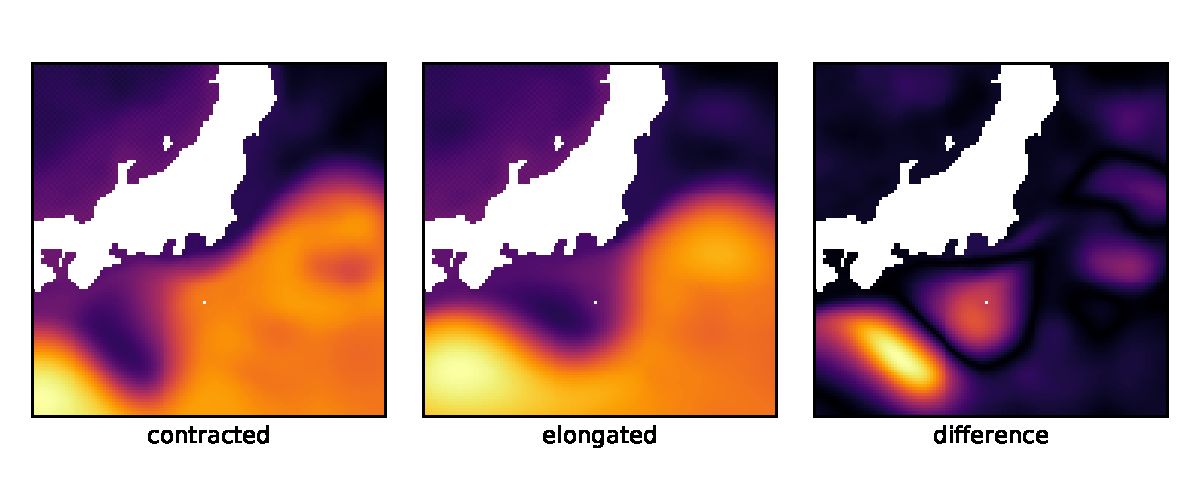
\includegraphics[width=\linewidth]{kuroshio_elon_contr.pdf}
  \caption{The two distinct states of the Kuroshio created by averaging SSH over
  two years. The images have a size of 100 x 100 which are sliced out of the global
  simulation domain of 3600 x 2400 pixels.}
  \label{fig:kuroshio_elon_contr}
\end{figure}

\begin{figure}
  \centering
  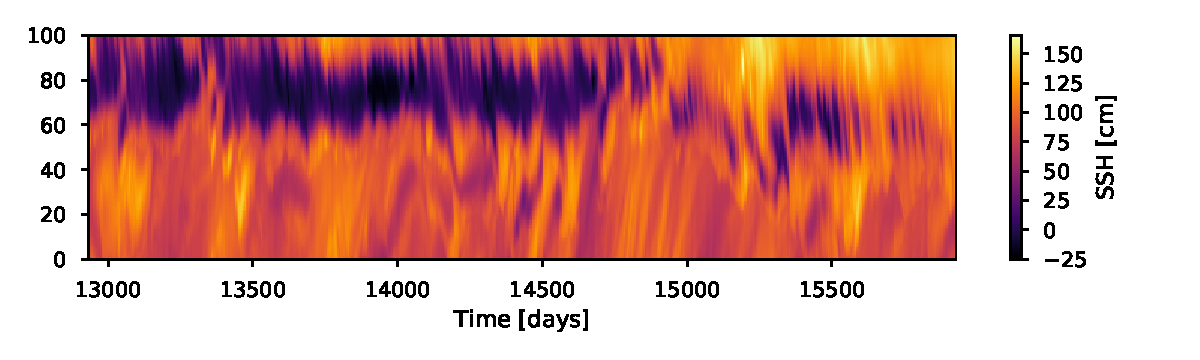
\includegraphics[width=\linewidth]{kuroshio_evolution.pdf}
  \caption{A row of the southern SSH field from
  Fig.~\ref{fig:kuroshio_elon_contr} over time.  The Kuroshio anomaly where
  the stream transitions from contracted to elongated state is visible between
  day 14500 and 15000.
  }
  \label{fig:kuroshio_evolution}
\end{figure}

Detecting the state changes of the Kuroshio with an automated anomaly search
could be the first step in creating a way of finding novel behaviour in the
vast amount of climate model output, which is essentially as unexplored as the
oceans of our real world.  Such novelties could, apart from their potential of
displaying new physical processes, contribute both to a further understanding
of the behaviour of the Kuroshio itself and the ocean circulation patterns as a
whole.  The automatic detection of the Kuroshio anomaly would mark a major step
towards a creation of an algorithm that could find anomalies in noisy and
turbulent datasets such as ocean simulations.
